\documentclass{article}
\usepackage[margin=1in]{geometry}
\usepackage{../common}
\usepackage{../pagesetup}

\begin{document}

\lecture{10}{September 11}{Sasha Rush}{Max Hopkins, Sebastian Wagner-Carena, Mien Wang, Jamila Pegues}{Exact Inference: Time Series}

\section{Prelude}
\subsection{Notation}
Recall from Lecture 9 our notation for the joint probability distributions of \textit{Undirected Graphical Models} (UGMs). In particular, we have
\[
p(x_1,\ldots,x_T)=exp\{\sum\limits_c \theta_c(x_c) - A(\theta)\}
\]
Here, $\theta_c(x_c)$ is the score associated with some clique $c$, and $x_c$ is some value assignment on the clique. This notation is great because it corresponds to exponential families! However, there are a few other notations you may see around:
\begin{align*}
p(x_1,\ldots,x_T) &\propto \prod\limits_c exp(\theta_c(x_c))\\
&= \prod\limits_c \psi_c(x_c))
\end{align*}
This latter notation is used by Murphy. $\psi_c(x_c)$ are the potentials, and they are simply exp$(\theta_c(x_c)$. The score functions $\theta_c$ are then known as the log potentials.
\subsection{Moralization}
Recall from last lecture the process of conversion between a \textit{Directed Graphical Model} (DGM) and UGM, known as moralization. Here we consider two diagrams:
\begin{center}
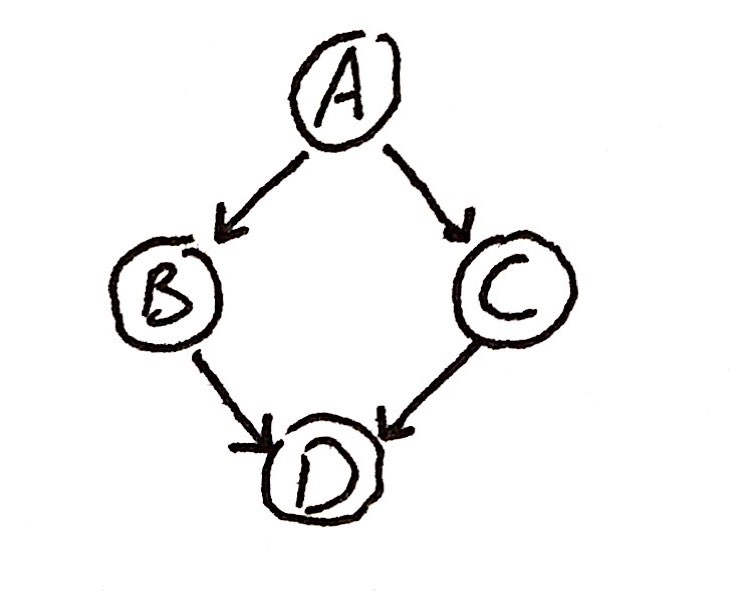
\includegraphics[scale=.15]{DGM1}
\end{center}
The first has joint probability distribution
\[
P(A,B,C,D)=P(A)P(B|A)P(C|A)P(D|B,C)
\]
After moralization, we have
\begin{center}
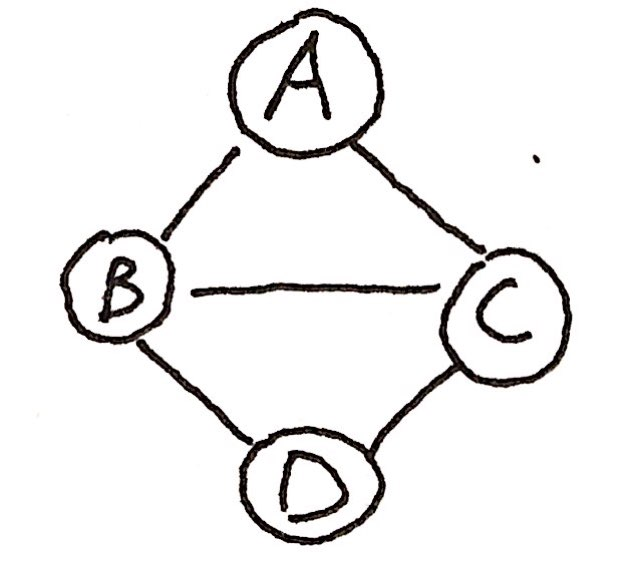
\includegraphics[scale=.15]{UGM1}
\end{center}
We see that the UGM has two cliques, the $c_0=\{A,B,C\}$, and $c_1=\{B,C,D\}$.
Using the notation above, this gives us
\[
P(A,B,C,D) = \psi_{c_0}(A,B,C)\psi_{c_1}(B,C,D)
\]
This form gives a particularly nice parallelism where it is clear that the first three terms 
\[
P(A)P(B|A)P(C|A)=\psi_{c_0}(A,B,C)
\]
and
\[
P(D|B,C)=\psi_{c_1}(B,C,D)
\]
\subsection{Conditional Independence vs. Parametrization}
It is important to keep in mind that DGMs only specify conditional independence. The same DGM's could correspond to completely different parametrizations of the random variables. For example, consider Naive Bayes:
\begin{center}
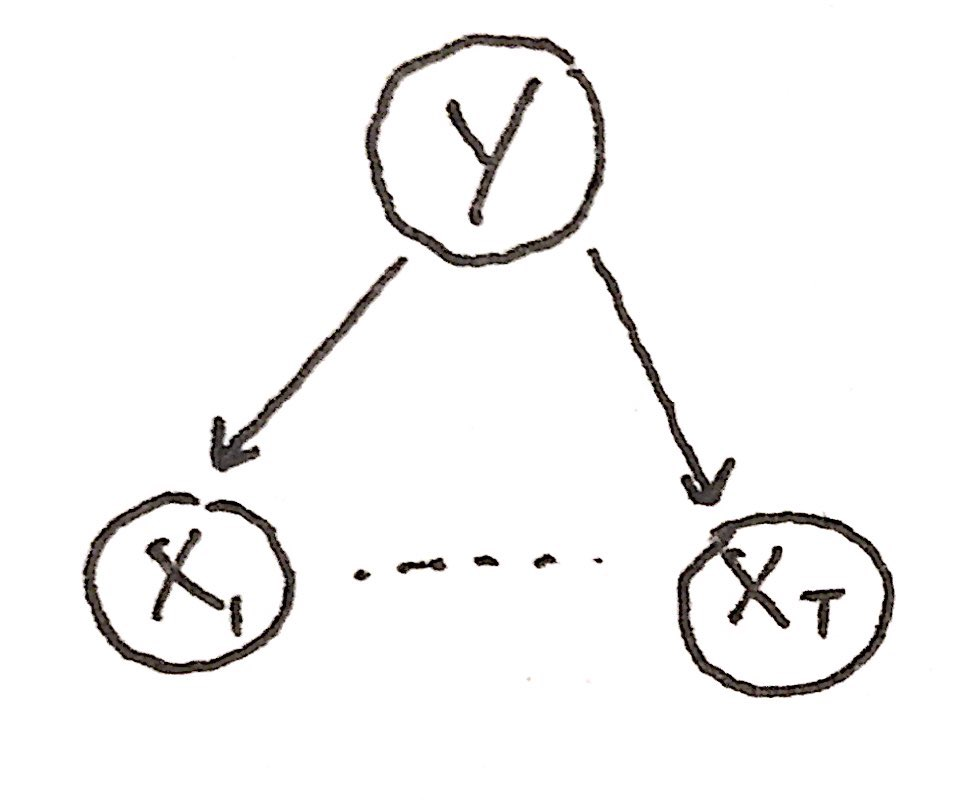
\includegraphics[scale=.1]{naive_bayes}
\end{center}
In Lecture 5, we discussed all kinds of Naive Bayes (NB), including Bernoulli, MVN, Categorical, and more. All of these follow the diagram above, which only specifies the conditional probability distribution
\[
p(x|y)=p(y)\prod\limits_i p(x_i|y)
\]
Now consider a conditional model:
\begin{center}
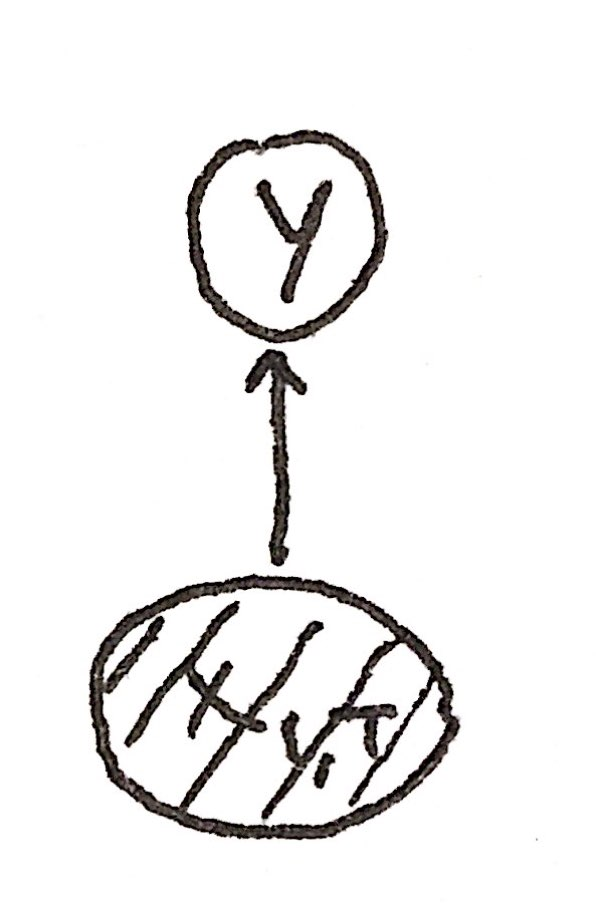
\includegraphics[scale=.1]{conditional_diagrams}
\end{center}
Here we are only interested in $p(y|x_1,\ldots,x_T)$. Similarly to NB, the parametrizations of this model can take many forms. For instance, one could use logistic or linear regression, most GLM's, Neural Networks, or even convolutional Neural Networks. In fact this is the model on which Alphago functions, where features $x$ are the tile placements on the board, and $y$ is the output move!

The main point here is that we can stick arbitrary parametrizations into graphical models. These diagrams just specify the conditional dependence--not the distributions. Further, as long as we specify the graphical model structure, we will be able to tell how hard inference will be.
\section{Time Series}
In this lecture, we only consider an informal definition of a time series. This structure is marked by collecting data over time, and predicting an output for each data input.
We are going to consider a special case, labeling a time series. Here our we will have $x_{1:T}$ as our input sequence (features), and $y_{1:T}$ as our output labels. We will begin by providing examples of labeling time series:
\begin{example}[OCR]
Here we have blocks of pixels, discrete vectors, each which depict a letter. These blocks are our $x_i$, and each corresponding $y_i$ the discrete symbol the $x_i$ represents
\begin{center}
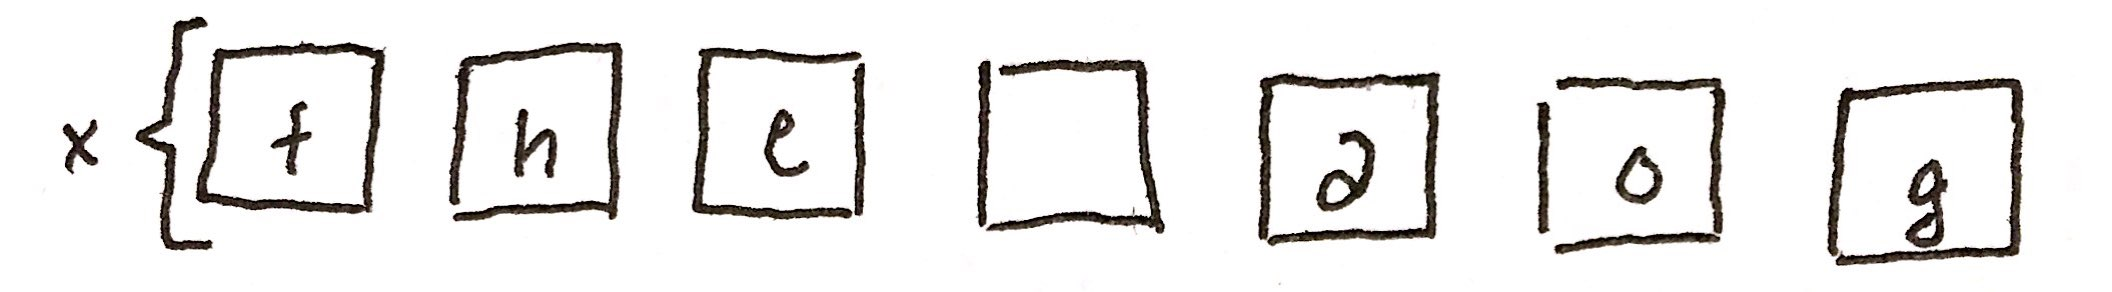
\includegraphics[scale=.1]{OCR} \\
y = \{t,h,e, ,d,o,g\}
\end{center}
\end{example}
\begin{example}[NLP]
Here we are given discete words as input variables $x$, and we wish to predict discrete $y$, their parts of speech
\begin{center}
x: the dog ate a carrot \\
y: DT NOUN VERB DT NOUN
\end{center}
\end{example}
\begin{example}[Speech Recognition]
Recall from previous lectures that our signal may be divided up into time steps and translated to continues vectors in $\R^{13}$, these our are continuous input variables $x$. Our output for each vector is the phoneme corresponding to the sound.
\begin{center}
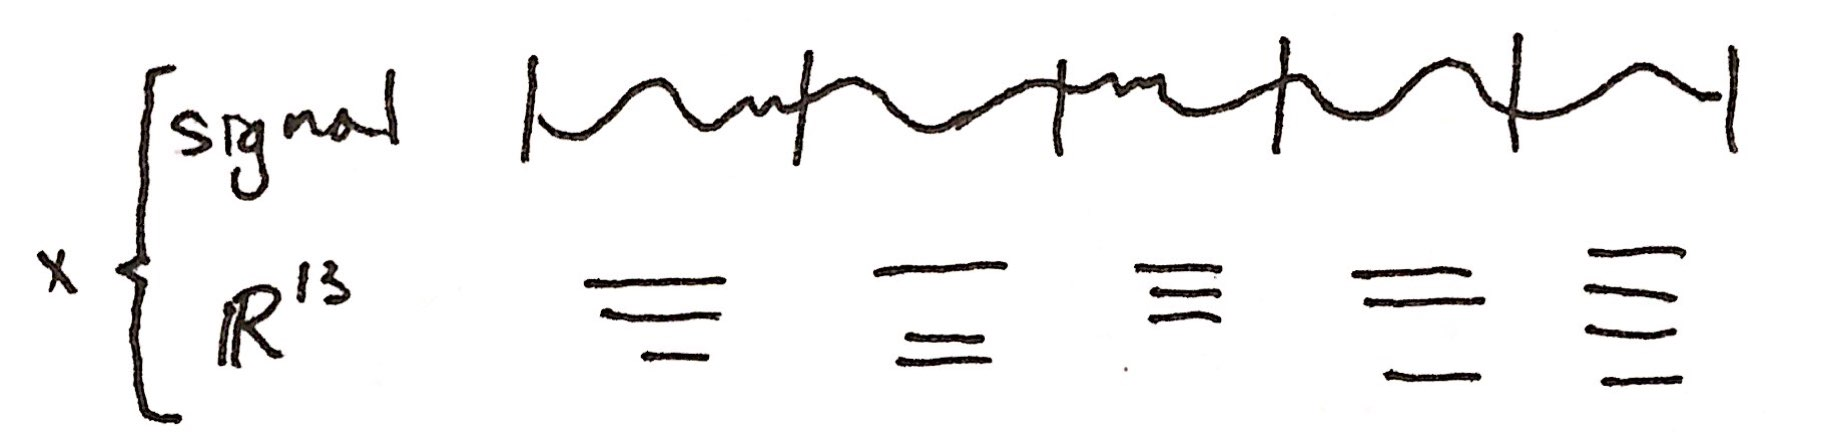
\includegraphics[scale=.1]{SpeechRec} \\
y = \{d,d,d,o,o\}
\end{center}
\end{example}
\begin{example}[Tracking]
Here we are tracking the position of some object with presumed Gaussian noise. In this case both our input and output variables are continuous. The inputs are our position vectors, and the output is the predicted correction for noise.
\begin{center}
\includegraphics[scale=.1]{Tracking} 
\end{center}
\end{example}
\begin{example}[Education]
This example is based upon the presentation at the beginning of the class. Our inputs are given by a kinect tracker and are continuous body positions at snapshots in time. The discrete output y is whether the body position corresponds to attentive or bored.
\begin{center}
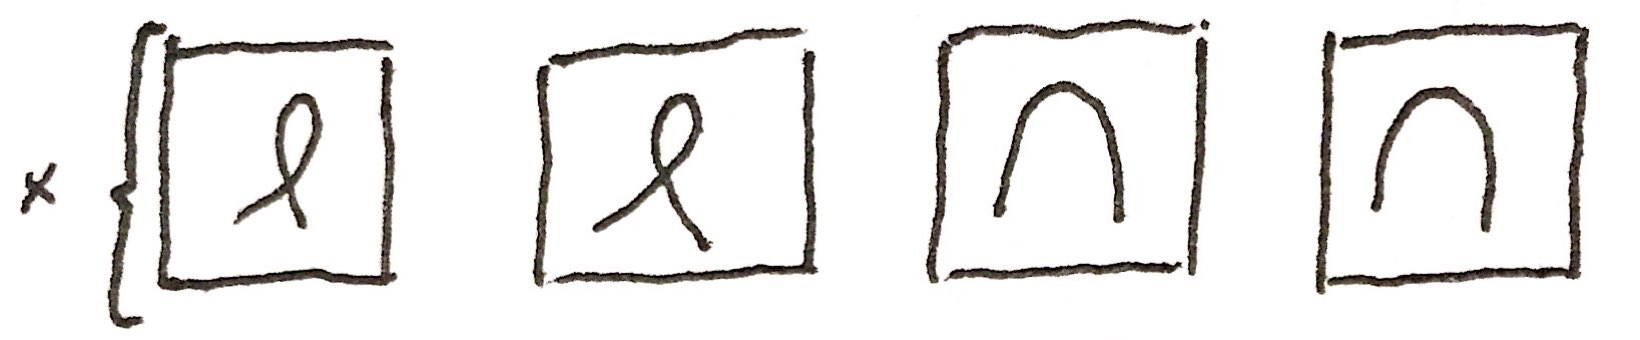
\includegraphics[scale=.1]{education} \\
y = \{attentive, attentive, bored, bored \}
\end{center}
\end{example}
\begin{example}[Touch-typing]
We consider typing on an iphone, where inputs are the continuous position of keystrokes on the phone. The outputs y are given by discrete letters.
\begin{center}
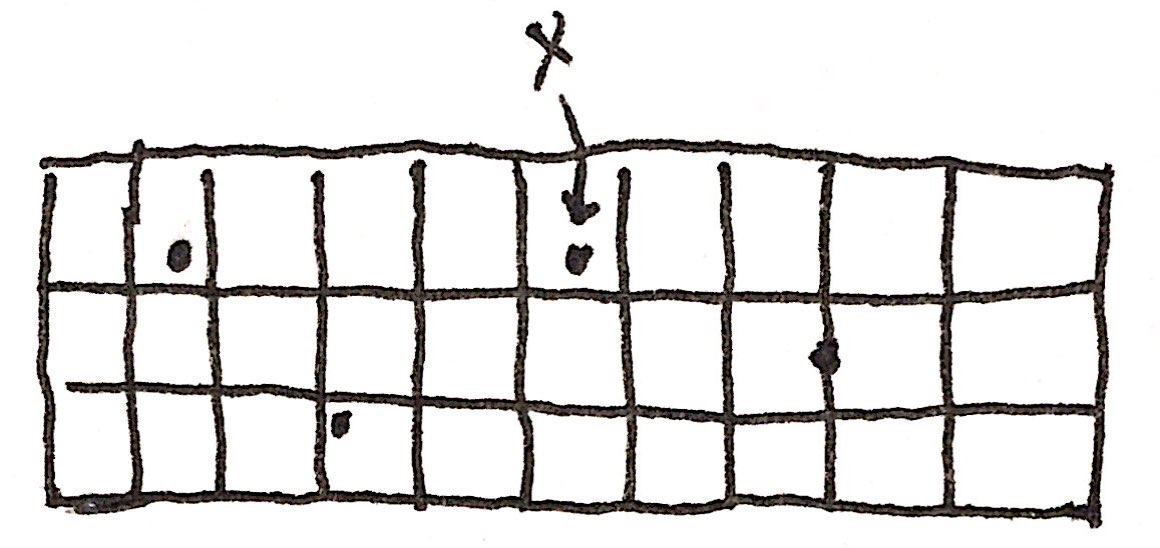
\includegraphics[scale=.1]{TouchTyping} \\
y = \{s,t,o,p\}
\end{center}
\end{example}
\section{Markov Models}
\subsection{Hidden Markov Model}
\begin{center}
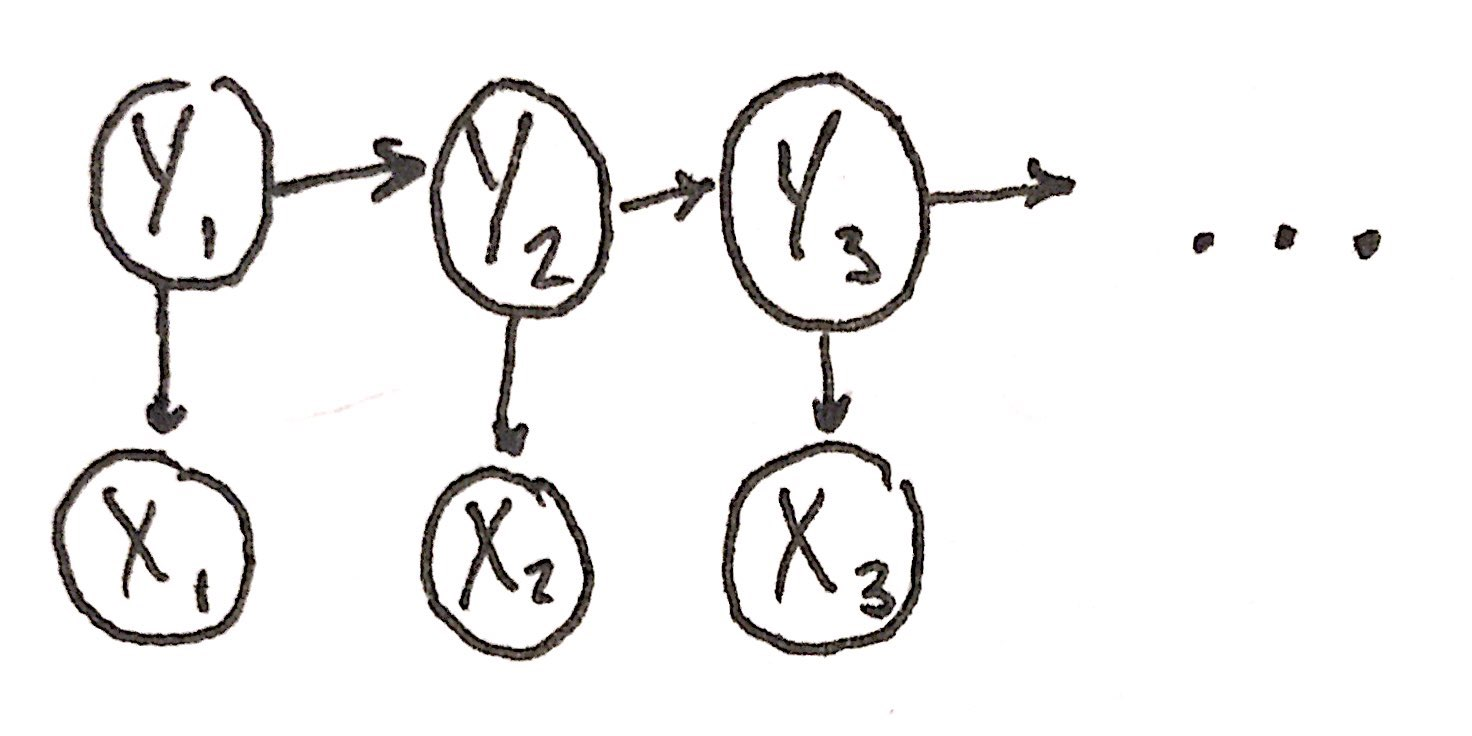
\includegraphics[scale=.1]{HMM} 
\end{center}
We discussed several \textit{Markov Models} in previous lectures. We begin with the \textit{Hidden Markov Model} (HMM), which actually predates DGMs. HMMs assume discrete $y$, though DGMs with the same structure may have continuous $y$. This has a fully joint parametrization $p(y_{1:T},x_{1:T})$, where in most cases $p(y_t | y_{t-1})$ is categorical. We can choose the distribution of $p(x_i|y_i)$ to fit our given circumstances:
\begin{enumerate}
\item $p(x_i|y_i)$ is categorical [e.g. parts of speech]
\item $p(x_i|y_i)$ is MVN [typing, speech (this uses a mixed gaussian)]
\item $p(x_{i1},\ldots,x_{iv}|y_i) = \prod\limits_v p(x_{iv} | y_i)$ [OCR]
\end{enumerate}
The last example here has an embedded Naive Bayes model for each feature $x$. 
\begin{center}
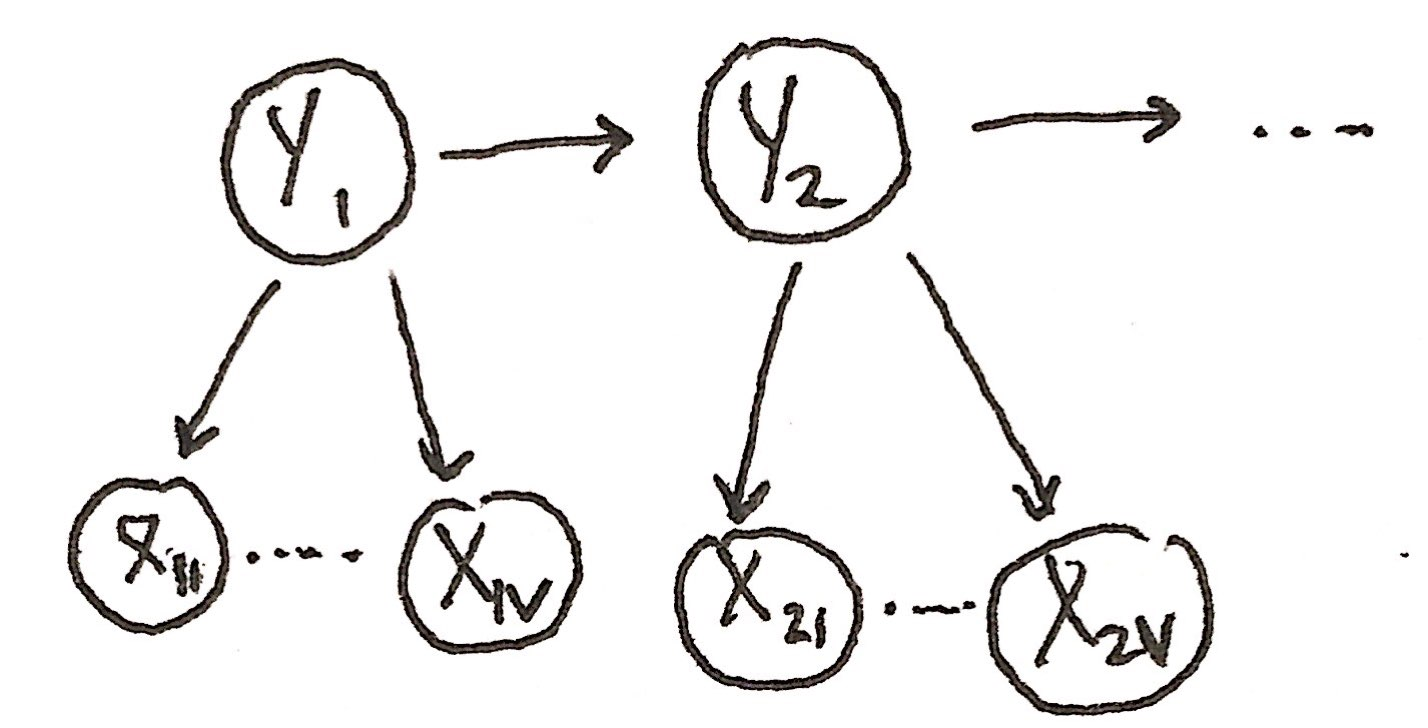
\includegraphics[scale=.1]{HMM_NB} 
\end{center}
HMMs such as the above are often parametrized in the following manner:
\begin{center}
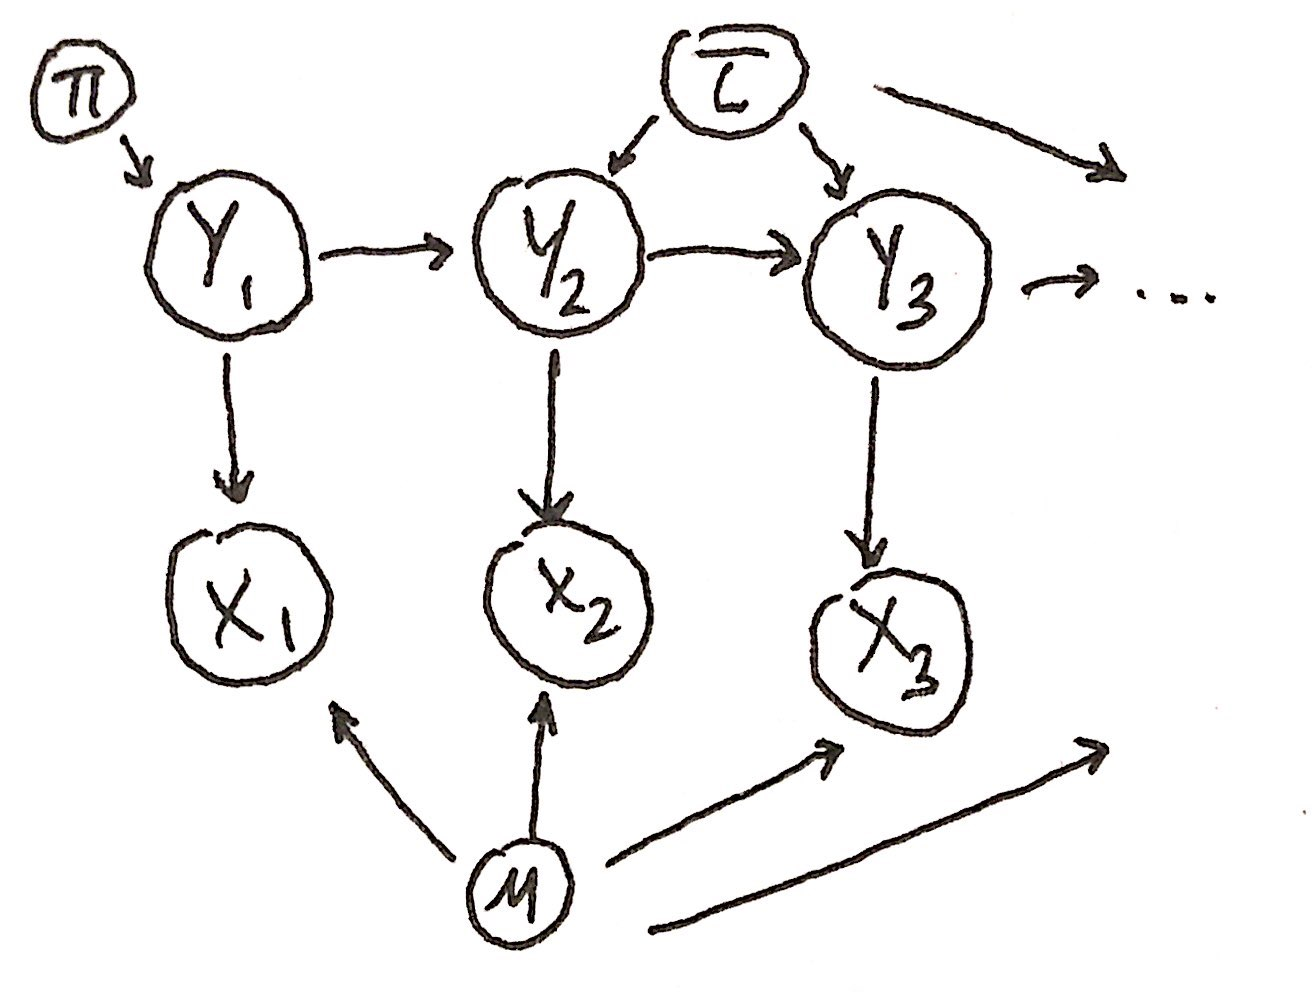
\includegraphics[scale=.1]{HMM_Param} 
\end{center}
\subsection{State Space Model}
While continuous y has the same graphical model, it has completely different usage and was developed completely separately. This model is called the \textit{State Space Model} (SSM). This model is often used when we have a continuous signal disturbed by gaussian noise--this becomes multivariate and we can compute inference nicely. 
\subsection{Maximum Entropy Markov Model}
Yet another Markov Model is the \textit{Maxent Markov Model} (MEMM). This model assumes we have observed all features, and flips the direction of the conditioning in the vertical direction.
\begin{center}
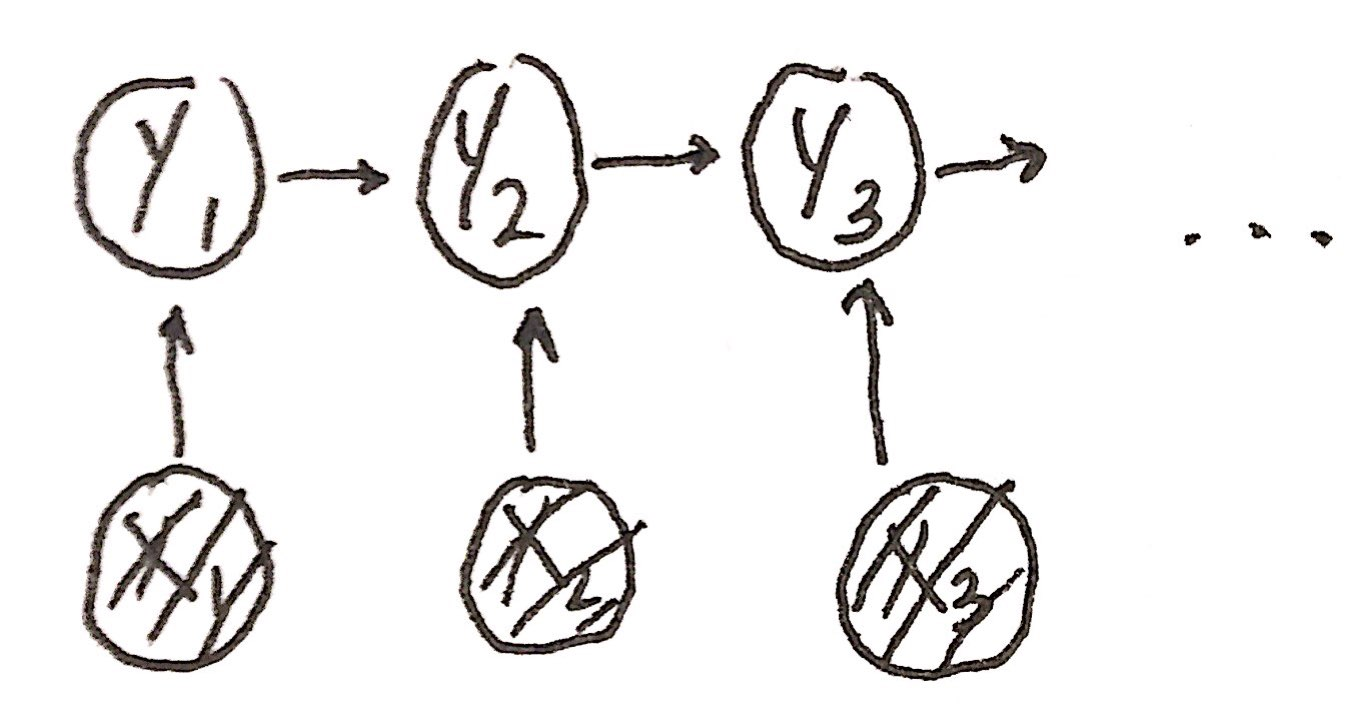
\includegraphics[scale=.1]{MEMM} 
\end{center}
Thus we are interested in $p(y_1,\ldots,y_T | x_1, \ldots, x_T)$, and $p(y_t|x_t,y_{t-1})$ is a GLM such as logistic or softmax regression.

MEMM comes with the distinct advantage that we no longer have to assume our features are independent. This is particularly useful in, say, tagging parts of speech where can pick an arbitrary feature basis without worrying about independence. However, the model comes with the downside that there is no closed form, so we must use SGD, i.e. we isolate each $x_i$ and predict $y_i$ with logistic regression.

Picking $p(y_t|x_t,y_{t-1})$ here as an arbitrary neural network is called a Neural Network Markov Model or NN-Markov Model. 
\section{Conditional Random Field Markov Model}
While CRF is still a Markov Model, it gets its own section due to its importance. The CRF is simply the UGM of all the above Markov Models:
\begin{center}
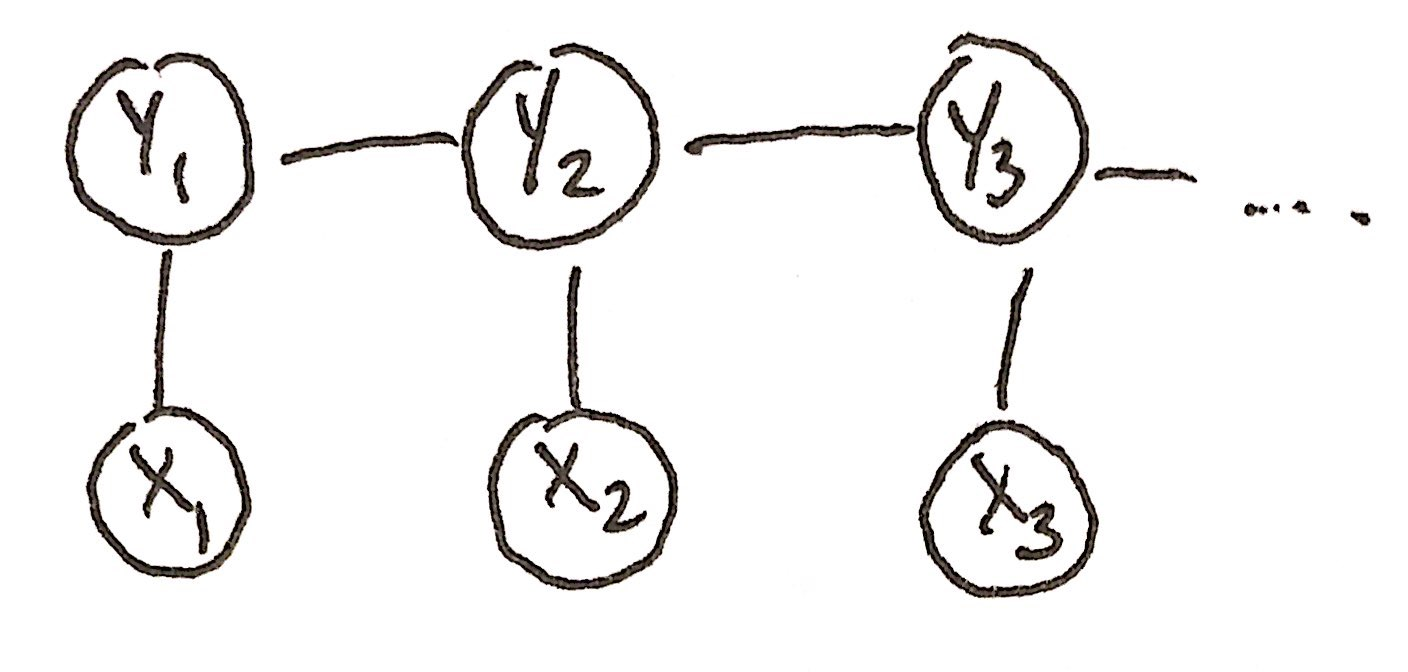
\includegraphics[scale=.1]{CRF} 
\end{center}
Recalling Subsection 1.1, we write
\[
p(y_{1:T}|x_{1:T} = exp\{\sum\limits_{t}(\theta_t^h(y_t,y_{t-1})+\theta_t^o(y_t,x_t)) - A(\theta) \}
\]
Here $h$ and $o$ refer to the labeled arrows in the diagram.
This is the general form of any Markov Model. Note that because we have observed the features $x_{1:T}$, we may rewrite the $T_t^o(y_t,x_t)$ terms as $\theta_t^o(y_t;x_t)$. If we are trying to do inference, we can think of the above after conditioning as simply
\begin{center}
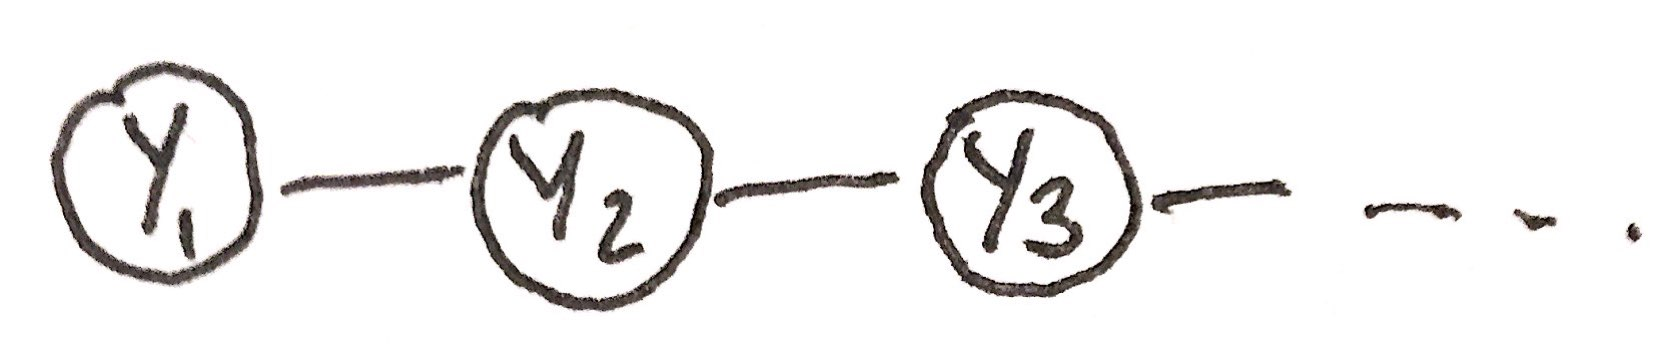
\includegraphics[scale=.1]{M_chain} 
\end{center}
This is a simple \textit{Markov Chain} UGM. In fact after converting to UGM and conditioning on our features, all Markov models become the above! 

Now while we can compute the closed form of the MLE on HMMs, CRF is a bit tricker. However, it is a member of the exponential family model, and we know the MLE for these families in general.
\[
\mathbb{E}(\phi(x)) = \frac{\sum \phi(x_d)}{N}
\]
Here, $\phi(y)$ are the sufficient statistics--but what do these look like? In fact we went over this in a previous lecture, it is simply a vector of indicator functions for every clique assignment (see Lecture 9). For inference in particular, we care about
\[
\mathbb{E}(\textbf{1}(x_c=v))
\]
Then the clique marginals are given by
\[
\frac{\sum\limits_{x'=x'_c=v} p(x')}{\sum\limits_{x''}p(x'')}
\]
However this may be computationally intractable, as the $x''$ we sum over is the entire universe! However, this can be computed efficiently for some models such as chain models

\section{Bonus: Lecture by Bertrand Schnieder}

Bertrand Schnieder gave a snazzy guest lecture on his research, and advertised that the datasets from his research would be ideal as a base for CS 281 final projects.  We take a moment to review his lecture below.

Schnieder was very interested in studying patterns across concepts of collaborative learning. For example, joint attention refers to when a group of individuals are focused on the same physical object, and is an important part of language development. Signs of joint attention can be seen in the physical movement of the individuals involved, such as their eye movements, gestures, and body postures. 

Schnieder discussed studies that he and others carried out to explore joint attention. For example, one study gave forty-two pairs of two participants a task to solve, within a total of forty-five minutes of time. Over that time period, Schnieder et al. used high-frequency and multi-modal sensors to track different aspects of movement, including: video, audio, eye movement (tracked at 60Hz), physiological data (like heart rate; tracked at 1-30Hz), and even body posing and coordination (using a Kinect; tracked at 30Hz). Schnieder pointed out that these sorts of studies provide massive amounts of data. During the lecture, he highlighted that there are a number of cool CS 281 projects that could arise from datasets like this one. Some projects he proposed are:
\begin{enumerate}

\item Unsupervised machine learning: modeling collaborative learning processes with probabilistic graphical models.
\item Supervised machine learning: training models to make predictions. For instance, training a model to predict the joint visual attention of two people based on their gestures, head orientation, and speech. Another example is training a model to predict physiological activity based on features like pupil size and body posture. With supervised machine learning, however, Schnieder noted that overfitting can be a dangerous pitfall.
\item Design your own!

\end{enumerate}

Schnieder emphasized that he is open to ideas, and that he highly encourages anyone interested in working with this data in some way or form to email him at bertrand\_schneider@gse.harvard.edu.

\end{document}

